\documentclass[12pt,a4paper]{article}

% --- Page Layout -------------------------------------------------------------
\usepackage[a4paper, margin=0.8in, headheight=14pt]{geometry}

% --- Fonts (XeLaTeX) ---------------------------------------------------------
\usepackage{fontspec}
\usepackage{unicode-math}
\setmainfont{TeX Gyre Pagella}
\setmonofont[Scale=0.88]{TeX Gyre Cursor}
\setmathfont{Latin Modern Math}

% --- Packages ---------------------------------------------------------------
\usepackage{xcolor}
\usepackage{titlesec}
\usepackage{enumitem}
\usepackage{tabularx}
\usepackage{booktabs}
\usepackage{array}
\usepackage{amsmath}
\usepackage{tikz}
\usetikzlibrary{shapes.geometric, arrows.meta, positioning, calc, fit, decorations.pathreplacing}
\usepackage{tcolorbox}
\tcbuselibrary{skins, breakable}
\usepackage{hyperref}
\usepackage{fancyhdr}
\usepackage{graphicx}
\usepackage{microtype}
\hyphenpenalty=10000
\exhyphenpenalty=10000
\sloppy
\usepackage{caption}
\usepackage{setspace}
\usepackage{multirow}
\usepackage{tocloft}

% --- Q&A helper --------------------------------------------------------------
\newcommand{\Q}[1]{\textbf{#1}\par\noindent\ignorespaces}

% --- Colour Palette ----------------------------------------------------------
\definecolor{myred}{RGB}{196,30,58}
\definecolor{mydark}{RGB}{30,30,50}
\definecolor{mygreen}{RGB}{14,120,80}
\definecolor{myteal}{RGB}{0,130,140}
\definecolor{myamber}{RGB}{180,100,0}
\definecolor{mypurple}{RGB}{100,30,160}
\definecolor{mygray}{RGB}{246,247,249}
\definecolor{mgframe}{RGB}{180,185,200}
\definecolor{watermark}{RGB}{145,150,170}
\definecolor{hdrred}{RGB}{250,232,235}
\definecolor{hdrgreen}{RGB}{220,244,233}
\definecolor{hdrteal}{RGB}{220,242,244}
\definecolor{hdramber}{RGB}{253,242,215}
\definecolor{hdrpurple}{RGB}{238,228,255}
\definecolor{hdrgray}{RGB}{238,240,245}
\definecolor{rowalt}{RGB}{250,251,253}

% --- Section Formatting ------------------------------------------------------
\titleformat{\section}
  {\large\bfseries\color{myred}}{\thesection.}{0.5em}{}
  [\vspace{1pt}{\color{myred}\rule{\linewidth}{0.8pt}}]
\titleformat{\subsection}
  {\normalsize\bfseries\color{myteal}}{\thesubsection}{0.5em}{}
\titlespacing*{\section}{0pt}{18pt}{7pt}
\titlespacing*{\subsection}{0pt}{11pt}{4pt}

% --- Paragraph ---------------------------------------------------------------
\setlength{\parindent}{0pt}
\setlength{\parskip}{4pt}

% --- TOC Styling -------------------------------------------------------------
\renewcommand{\cfttoctitlefont}{\large\bfseries\color{myred}}
\renewcommand{\cftaftertoctitle}{\par\noindent{\color{myred}\rule{\linewidth}{0.8pt}}}
\setlength{\cftbeforetoctitleskip}{0pt}
\setlength{\cftaftertoctitleskip}{6pt}
\renewcommand{\cftsecfont}{\normalsize\bfseries\color{mydark}}
\renewcommand{\cftsecpagefont}{\normalsize\bfseries\color{mydark}}
\renewcommand{\cftsecleader}{\cftdotfill{\cftdotsep}}
\setlength{\cftbeforesecskip}{7pt}
\renewcommand{\cftsubsecfont}{\small\color{mydark}}
\renewcommand{\cftsubsecpagefont}{\small\color{mydark}}
\setlength{\cftbeforesubsecskip}{3pt}
\setlength{\cftsubsecindent}{1.4em}

% --- Table helpers -----------------------------------------------------------
\renewcommand{\arraystretch}{1.45}
\setlength{\tabcolsep}{6pt}
\newcolumntype{B}[1]{>{\small\bfseries\raggedright\arraybackslash}m{#1}}
\newcolumntype{Y}{>{\small\raggedright\arraybackslash}X}
\renewcommand{\tabularxcolumn}[1]{m{#1}}

% --- Header / Footer ---------------------------------------------------------
\pagestyle{fancy}
\fancyhf{}
\fancyhead[L]{\small\color{myred}\textbf{BS-CH101}\;\color{mydark}--- Chemistry-I}
\fancyhead[R]{\small\color{myteal}\textbf{Module 7 Notes}}
\fancyfoot[C]{\small\color{mydark}\thepage}
\fancyfoot[R]{\small\color{watermark}\textit{\copyright\ Biraj}}
\renewcommand{\headrulewidth}{0.5pt}
\renewcommand{\footrulewidth}{0.3pt}

% --- Hyperref ---------------------------------------------------------------
\hypersetup{
  colorlinks=true, linkcolor=myteal, urlcolor=myteal,
  pdfauthor={Biraj Sarkar},
  pdftitle={BS-CH101 --- Module 7 Notes}
}

% --- tcolorbox styles --------------------------------------------------------
\tcbset{
  tikzbox/.style={
    colback=mygray, colframe=mgframe, boxrule=0.6pt, arc=4pt,
    left=8pt, right=8pt, top=6pt, bottom=6pt,
    colbacktitle=mgframe, coltitle=mydark,
    fonttitle=\small\bfseries
  },
  defbox/.style={
    colback=hdrgreen, colframe=mygreen, boxrule=0.8pt, arc=4pt,
    left=9pt, right=9pt, top=6pt, bottom=6pt,
    colbacktitle=mygreen, coltitle=white,
    fonttitle=\small\bfseries
  },
  formulabox/.style={
    colback=hdrteal, colframe=myteal, boxrule=0.8pt, arc=4pt,
    left=9pt, right=9pt, top=7pt, bottom=7pt,
    colbacktitle=myteal, coltitle=white,
    fonttitle=\small\bfseries
  },
  examplebox/.style={
    colback=hdramber, colframe=myamber, boxrule=0.8pt, arc=4pt,
    left=9pt, right=9pt, top=6pt, bottom=6pt,
    colbacktitle=myamber, coltitle=white,
    fonttitle=\small\bfseries
  },
  masonbox/.style={
    colback=hdrpurple, colframe=mypurple, boxrule=0.8pt, arc=4pt,
    left=9pt, right=9pt, top=6pt, bottom=6pt,
    colbacktitle=mypurple, coltitle=white,
    fonttitle=\small\bfseries
  },
  exambox/.style={
    colback=hdrpurple, colframe=mypurple, boxrule=1pt, arc=5pt,
    left=10pt, right=10pt, top=8pt, bottom=8pt,
    colbacktitle=mypurple, coltitle=white,
    fonttitle=\bfseries,
    breakable, title after break={\textbf{Frequently Asked / Viva Questions (contd.)}}}
}
\tcbset{breakable}

% --- TikZ styles -------------------------------------------------------------
\tikzset{
  block/.style={rectangle, draw=myteal, fill=hdrteal,
    text width=2.4cm, align=center, minimum height=0.95cm,
    font=\small, rounded corners=3pt, line width=0.7pt},
  redblock/.style={rectangle, draw=myred, fill=hdrred,
    text width=2.4cm, align=center, minimum height=0.95cm,
    font=\small, rounded corners=3pt, line width=0.7pt},
  netnode/.style={rectangle, draw=myteal, fill=hdrteal,
    text width=1.5cm, align=center, minimum height=0.8cm,
    font=\small, rounded corners=3pt, line width=0.7pt},
  sumjunc/.style={circle, draw=myamber, fill=hdramber,
    minimum size=0.62cm, font=\small, line width=0.8pt},
  snode/.style={circle, draw=mypurple, fill=hdrpurple,
    minimum size=0.55cm, font=\footnotesize, line width=0.7pt},
  arrow/.style={-Stealth, thick, color=mydark},
  redarrow/.style={-Stealth, thick, color=myred},
  line/.style={thick, color=mydark}
}

\begin{document}

\begin{center}
  {\LARGE\bfseries\color{myred} BS-CH101 / BS-CH201 --- Chemistry-I}\\[5pt]
  {\normalsize\color{mydark} Semester I \quad$\bullet$\quad 3L:1T:0P \quad$\bullet$\quad 4 Credits}\\[3pt]
  {\normalsize\color{myteal}\textbf{Module 7 Exam Notes: Organic Reactions and Drug Molecule Synthesis}}\\[3pt]
  {\small\color{mydark} CGEC \;$|$\; B.Tech ECE (2023--27) \;$|$\; \textit{Biraj Sarkar}}
\end{center}
\vspace{2pt}
\noindent{\color{myred}\rule{\linewidth}{1.5pt}}
\vspace{2pt}

\hypersetup{linkcolor=mydark}
\tableofcontents
\hypersetup{linkcolor=myteal}
\newpage
% ===============================================================================
\section{Organic Reactions and Drug Molecule Synthesis}
% ===============================================================================

\begin{tcolorbox}[defbox]
\textbf{Organic reaction mechanism} explains the step-by-step breaking and making of bonds during conversion of reactants into products. It identifies intermediates, reagents, and electron movement.
\end{tcolorbox}

\subsection{Substitution Reactions}
In substitution, one atom or group is replaced by another. Nucleophilic substitution is common in alkyl halides.

\begin{tabularx}{\linewidth}{|B{2.8cm}|Y|Y|}
\hline
\textbf{Type} & \textbf{Main feature} & \textbf{Favoured by} \\
\hline
$\mathrm{S_N1}$ & Two-step, carbocation intermediate & Tertiary substrate, polar protic solvent \\
\hline
$\mathrm{S_N2}$ & One-step backside attack & Methyl/primary substrate, strong nucleophile \\
\hline
\end{tabularx}

\begin{tcolorbox}[tikzbox, title={SN2 Backside Attack Concept}]
\centering
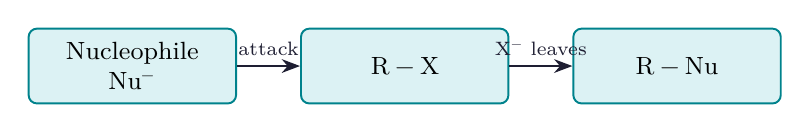
\begin{tikzpicture}[node distance=1.0cm and 0.8cm]
  \node[block] (nu) {Nucleophile\\$\mathrm{Nu^-}$};
  \node[block, right=of nu] (rx) {$\mathrm{R-X}$};
  \node[block, right=of rx] (prod) {$\mathrm{R-Nu}$};
  \draw[arrow] (nu) -- node[above,font=\scriptsize] {attack} (rx);
  \draw[arrow] (rx) -- node[above,font=\scriptsize] {$\mathrm{X^-}$ leaves} (prod);
\end{tikzpicture}
\end{tcolorbox}

\subsection{Addition and Elimination Reactions}
Addition reactions add atoms across multiple bonds. Elimination reactions remove atoms from adjacent carbons to form a double bond.

\begin{tcolorbox}[formulabox, title={Typical Patterns}]
\[
\mathrm{C=C + XY \rightarrow X-C-C-Y}
\]
\[
\mathrm{R-CH_2-CH_2X \rightarrow R-CH=CH_2 + HX}
\]
\end{tcolorbox}

\subsection{Oxidation, Reduction, Cyclization and Ring Opening}
Oxidation increases C-O, C-N, or C-X bonds or decreases C-H bonds. Reduction increases C-H bonds or removes electronegative atoms. Cyclization forms a ring; ring opening converts cyclic compounds into open-chain products.

\begin{tabularx}{\linewidth}{|B{3cm}|Y|Y|}
\hline
\textbf{Reaction} & \textbf{Meaning} & \textbf{Example idea} \\
\hline
Oxidation & Gain of oxygen or loss of hydrogen & Alcohol to aldehyde/acid \\
\hline
Reduction & Gain of hydrogen or loss of oxygen & Carbonyl to alcohol \\
\hline
Cyclization & Ring formation & Intramolecular attack \\
\hline
Ring opening & Cleavage of a ring bond & Epoxide hydrolysis \\
\hline
\end{tabularx}

\subsection{Synthesis of a Common Drug Molecule: Aspirin}
Aspirin (acetylsalicylic acid) is prepared by acetylation of salicylic acid using acetic anhydride in acidic medium.

\begin{tcolorbox}[formulabox, title={Aspirin Synthesis Reaction}]
\[
\mathrm{Salicylic\ acid + Acetic\ anhydride \xrightarrow{H^+} Aspirin + Acetic\ acid}
\]
\end{tcolorbox}

\begin{tcolorbox}[tikzbox, title={Flow Diagram for Aspirin Preparation}]
\centering
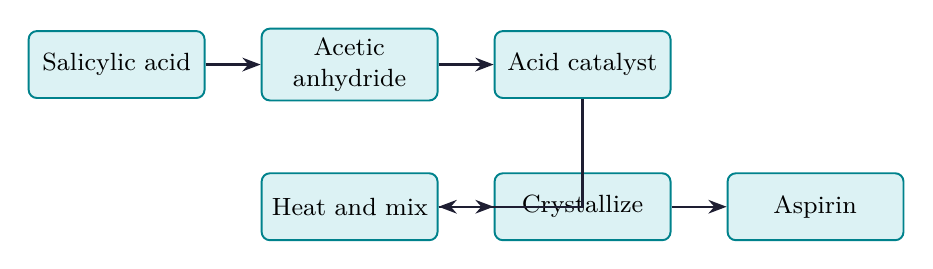
\begin{tikzpicture}[node distance=0.8cm and 0.7cm,
  sblock/.style={rectangle, draw=myteal, fill=hdrteal, text width=2.0cm,
    align=center, minimum height=0.85cm, font=\small,
    rounded corners=3pt, line width=0.7pt}]
  \node[sblock] (s1) {Salicylic acid};
  \node[sblock, right=of s1] (s2) {Acetic anhydride};
  \node[sblock, right=of s2] (s3) {Acid catalyst};
  \node[sblock, below=0.9cm of s2] (s4) {Heat and mix};
  \node[sblock, right=of s4] (s5) {Crystallize};
  \node[sblock, right=of s5] (s6) {Aspirin};
  \draw[arrow] (s1) -- (s2);
  \draw[arrow] (s2) -- (s3);
  \draw[arrow] (s3) |- (s4);
  \draw[arrow] (s4) -- (s5);
  \draw[arrow] (s5) -- (s6);
\end{tikzpicture}
\end{tcolorbox}

\subsection{Mechanistic Exam Language}
For mechanism-based answers, identify electrophile, nucleophile, leaving group, intermediate, and product. Use curved-arrow reasoning in words even when detailed curved arrows are not drawn.

\begin{tcolorbox}[exambox, title={Exam Points}]
\begin{itemize}[leftmargin=*, itemsep=2pt, topsep=2pt]
  \item Compare $\mathrm{S_N1}$ and $\mathrm{S_N2}$ using step, intermediate, rate law, and stereochemistry.
  \item For addition and elimination, write the general reaction pattern.
  \item For oxidation/reduction, state change in C-H and C-O bonds.
  \item For aspirin synthesis, mention salicylic acid, acetic anhydride, acid catalyst, and acetylation.
\end{itemize}
\end{tcolorbox}

% ===============================================================================
\section{Detailed Organic Reaction Notes and Synthesis Planning}
% ===============================================================================

\subsection{Reaction Intermediates}
Organic reactions often proceed through reactive intermediates. Stability of intermediates decides product distribution and rate.

\begin{tabularx}{\linewidth}{|B{3cm}|Y|Y|}
\hline
\textbf{Intermediate} & \textbf{Nature} & \textbf{Stability trend} \\
\hline
Carbocation & Electron-deficient carbon with positive charge & $3^\circ>2^\circ>1^\circ>\mathrm{CH_3^+}$ \\
\hline
Carbanion & Electron-rich carbon with negative charge & Stabilized by electron-withdrawing groups \\
\hline
Free radical & Species with unpaired electron & $3^\circ>2^\circ>1^\circ>\mathrm{CH_3\cdot}$ \\
\hline
Carbene & Neutral divalent carbon species & Highly reactive; addition to alkenes \\
\hline
\end{tabularx}

\subsection{Detailed Comparison of \texorpdfstring{$\mathrm{S_N1}$}{SN1} and \texorpdfstring{$\mathrm{S_N2}$}{SN2}}

\begin{tabularx}{\linewidth}{|B{3.0cm}|Y|Y|}
\hline
\textbf{Point} & \textbf{$\mathrm{S_N1}$} & \textbf{$\mathrm{S_N2}$} \\
\hline
Mechanism & Two-step & One-step concerted \\
\hline
Rate law & $k[\mathrm{RX}]$ & $k[\mathrm{RX}][\mathrm{Nu^-}]$ \\
\hline
Intermediate & Carbocation & No intermediate \\
\hline
Substrate & $3^\circ>2^\circ>1^\circ$ & methyl $>1^\circ>2^\circ$ \\
\hline
Solvent & Polar protic & Polar aprotic \\
\hline
Stereochemistry & Racemization possible & Inversion of configuration \\
\hline
\end{tabularx}

\begin{tcolorbox}[examplebox, title={Solved Concept: Choosing SN1 or SN2}]
Tertiary butyl chloride reacts with water mainly by $\mathrm{S_N1}$ because a stable tertiary carbocation can form and water is a weak nucleophile in polar protic medium. Methyl bromide reacts with $\mathrm{OH^-}$ mainly by $\mathrm{S_N2}$ because backside attack is unhindered.
\end{tcolorbox}

\subsection{Electrophilic Addition to Alkenes}
Alkenes undergo electrophilic addition because the pi bond is electron rich. Addition of HX follows Markovnikov rule in normal ionic addition.

\begin{tcolorbox}[defbox]
\textbf{Markovnikov rule:} In addition of HX to an unsymmetrical alkene, hydrogen attaches to the carbon already having more hydrogen atoms, and X attaches to the more substituted carbon.
\end{tcolorbox}

\begin{tcolorbox}[formulabox, title={Addition of HBr to Propene}]
\[
\mathrm{CH_3-CH=CH_2+HBr\rightarrow CH_3-CHBr-CH_3}
\]
The major product is 2-bromopropane due to formation of the more stable secondary carbocation.
\end{tcolorbox}

\subsection{Elimination: E1 and E2}
Elimination reactions form alkenes. E1 proceeds through carbocation; E2 occurs in one step with base removing beta-hydrogen as leaving group departs.

\begin{tabularx}{\linewidth}{|B{3cm}|Y|Y|}
\hline
\textbf{Point} & \textbf{E1} & \textbf{E2} \\
\hline
Steps & Two-step & One-step \\
\hline
Intermediate & Carbocation & None \\
\hline
Base strength & Weak base possible & Strong base required \\
\hline
Substrate & Tertiary favoured & Primary, secondary, tertiary possible \\
\hline
Stereochemical need & No strict anti requirement & Anti-periplanar H and leaving group preferred \\
\hline
\end{tabularx}

\subsection{Oxidation and Reduction Reagents}
Remembering reagent function is more useful than memorizing long mechanisms for basic engineering chemistry.

\begin{tabularx}{\linewidth}{|B{3cm}|Y|Y|}
\hline
\textbf{Reagent} & \textbf{Type} & \textbf{Common use} \\
\hline
$\mathrm{KMnO_4}$ & Strong oxidizing agent & Alkene oxidation, alcohol oxidation \\
\hline
$\mathrm{K_2Cr_2O_7/H^+}$ & Oxidizing agent & Primary alcohol to acid, secondary alcohol to ketone \\
\hline
$\mathrm{LiAlH_4}$ & Strong reducing agent & Carbonyl and acid derivatives to alcohols \\
\hline
$\mathrm{NaBH_4}$ & Mild reducing agent & Aldehyde/ketone to alcohol \\
\hline
$\mathrm{H_2/Ni}$ & Catalytic reduction & Alkene to alkane \\
\hline
\end{tabularx}

\subsection{Cyclization and Ring Opening}
Cyclization is favoured when the reacting ends of a molecule can form a stable five- or six-membered ring. Ring opening is important for strained rings like epoxides.

\begin{tcolorbox}[tikzbox, title={Cyclization and Ring Opening Concept}]
\centering
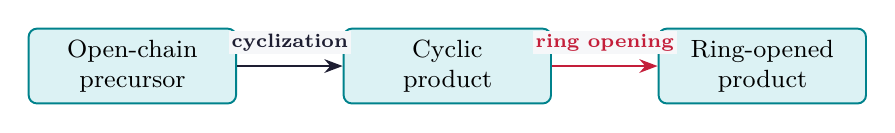
\begin{tikzpicture}[
  rxnlabel/.style={font=\scriptsize\bfseries, fill=mygray, inner sep=1pt}
]
  \node[block] (open) at (0,0) {Open-chain\\precursor};
  \node[block] (ring) at (4,0) {Cyclic\\product};
  \node[block] (open2) at (8,0) {Ring-opened\\product};
  \draw[arrow] (open) -- node[rxnlabel, above=4pt] {cyclization} (ring);
  \draw[redarrow] (ring) -- node[rxnlabel, above=4pt] {ring opening} (open2);
\end{tikzpicture}
\end{tcolorbox}

\subsection{Aspirin Synthesis: Mechanism and Purification}
In aspirin preparation, salicylic acid provides the phenolic $-\mathrm{OH}$ group and acetic anhydride provides the acetyl group. Acid catalyst increases electrophilicity of acetic anhydride. The product is purified by recrystallization.

\begin{enumerate}[leftmargin=*, itemsep=3pt, topsep=2pt]
  \item Protonation of acetic anhydride increases electrophilic character of carbonyl carbon.
  \item Phenolic oxygen of salicylic acid attacks the carbonyl carbon.
  \item Acetate group leaves and deprotonation gives aspirin.
  \item Cold water helps crystallize aspirin because aspirin is less soluble in cold water.
\end{enumerate}

\begin{tcolorbox}[examplebox, title={Aspirin Yield Calculation}]
If theoretical yield is $5.00\ \mathrm{g}$ and actual yield is $3.80\ \mathrm{g}$:
\[
\%\ \text{yield}=\frac{\text{actual yield}}{\text{theoretical yield}}\times100
\]
\[
\%\ \text{yield}=\frac{3.80}{5.00}\times100=76\%
\]
\end{tcolorbox}

\begin{tcolorbox}[masonbox, title={Organic Reaction Answer Checklist}]
\begin{enumerate}[leftmargin=*, itemsep=3pt, topsep=2pt]
  \item Identify substrate, reagent, nucleophile/electrophile, and leaving group.
  \item Classify the reaction as substitution, addition, elimination, oxidation, reduction, cyclization, or ring opening.
  \item Write rate law or regioselectivity rule where applicable.
  \item Mention major product and reason for its formation.
  \item For drug synthesis, include reactants, catalyst, reaction type, purification, and yield idea.
\end{enumerate}
\end{tcolorbox}

\subsection{Reaction Map for Basic Organic Transformations}
Most exam questions ask how one functional group changes into another. The following map gives the common first-year transformations.

\begin{tabularx}{\linewidth}{|B{3.2cm}|Y|Y|}
\hline
\textbf{Conversion} & \textbf{Typical reagent} & \textbf{Reaction class} \\
\hline
Alkene to alkane & $\mathrm{H_2/Ni}$ & Reduction / hydrogenation \\
\hline
Alkene to alcohol & $\mathrm{H_2O/H^+}$ & Addition \\
\hline
Alcohol to alkene & conc. $\mathrm{H_2SO_4}$, heat & Elimination / dehydration \\
\hline
Primary alcohol to acid & $\mathrm{KMnO_4}$ or $\mathrm{K_2Cr_2O_7/H^+}$ & Oxidation \\
\hline
Aldehyde to alcohol & $\mathrm{NaBH_4}$ & Reduction \\
\hline
Alkyl halide to alcohol & aqueous $\mathrm{KOH}$ & Nucleophilic substitution \\
\hline
\end{tabularx}

\subsection{Curly-Arrow Logic in Words}
Even when curved arrows are not drawn, the answer should describe electron flow clearly:
\begin{enumerate}[leftmargin=*, itemsep=3pt, topsep=2pt]
  \item A nucleophile donates an electron pair.
  \item An electrophile accepts an electron pair.
  \item A leaving group departs with the bonding electron pair.
  \item Formation of a stable intermediate or transition state controls the major product.
\end{enumerate}

\begin{tcolorbox}[examplebox, title={Worked Mechanism in Words: Alcohol to Alkene}]
In acid-catalysed dehydration of an alcohol, the $-\mathrm{OH}$ group is first protonated to form a better leaving group, water. Water leaves to form a carbocation. A base removes a beta-hydrogen, and a double bond forms. The major alkene is usually the more substituted alkene according to Zaitsev rule.
\end{tcolorbox}

\subsection{Zaitsev and Hofmann Elimination}
When more than one alkene can form, regioselectivity matters.

\begin{tabularx}{\linewidth}{|B{3cm}|Y|Y|}
\hline
\textbf{Rule} & \textbf{Major product} & \textbf{Typical condition} \\
\hline
Zaitsev rule & More substituted alkene & Small strong base or normal elimination \\
\hline
Hofmann rule & Less substituted alkene & Bulky base or quaternary ammonium elimination \\
\hline
\end{tabularx}

\subsection{Addition to Carbonyl Compounds}
The carbonyl group is polar. Carbon is electrophilic and oxygen is nucleophilic/basic. Nucleophiles attack the carbonyl carbon to form addition products.

\begin{tcolorbox}[tikzbox, title={Carbonyl Addition Concept}]
\centering
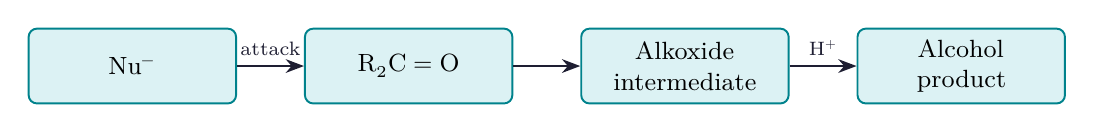
\begin{tikzpicture}[node distance=0.8cm and 0.85cm]
  \node[block] (nu) {$\mathrm{Nu^-}$};
  \node[block, right=of nu] (co) {$\mathrm{R_2C=O}$};
  \node[block, right=of co] (alk) {Alkoxide\\intermediate};
  \node[block, right=of alk] (alc) {Alcohol\\product};
  \draw[arrow] (nu) -- node[above,font=\scriptsize] {attack} (co);
  \draw[arrow] (co) -- (alk);
  \draw[arrow] (alk) -- node[above,font=\scriptsize] {$\mathrm{H^+}$} (alc);
\end{tikzpicture}
\end{tcolorbox}

\subsection{Green Chemistry Note for Drug Synthesis}
Engineering chemistry answers may include practical synthesis quality. A good drug synthesis should be high-yielding, selective, safe, and easy to purify.

\begin{tabularx}{\linewidth}{|B{3cm}|Y|}
\hline
\textbf{Green chemistry point} & \textbf{Meaning in aspirin synthesis} \\
\hline
Atom economy & Prefer maximum incorporation of reactant atoms into product \\
\hline
Safer solvent & Use minimum harmful solvent during purification \\
\hline
Energy efficiency & Avoid unnecessary heating time \\
\hline
Waste reduction & Reduce excess reagent and by-product handling \\
\hline
Product purity & Recrystallization improves purity for medicinal use \\
\hline
\end{tabularx}

\subsection{Tests for Functional Groups}
Short practical-style questions may ask how a functional group is detected.

\begin{tabularx}{\linewidth}{|B{3.2cm}|Y|Y|}
\hline
\textbf{Functional group} & \textbf{Test} & \textbf{Positive observation} \\
\hline
Alkene & Bromine water & Decolorization \\
\hline
Aldehyde & Tollens' reagent & Silver mirror \\
\hline
Carboxylic acid & Sodium bicarbonate & Brisk effervescence of $\mathrm{CO_2}$ \\
\hline
Phenol & Ferric chloride test & Violet or coloured complex \\
\hline
Alcohol & Esterification & Fruity smell of ester \\
\hline
\end{tabularx}

\begin{tcolorbox}[masonbox, title={Previous-Year Style Questions}]
\begin{enumerate}[leftmargin=*, itemsep=4pt, topsep=2pt]
  \item Compare $\mathrm{S_N1}$ and $\mathrm{S_N2}$ mechanisms with stereochemical outcome.
  \item Explain electrophilic addition to propene using Markovnikov rule.
  \item Compare E1 and E2 elimination reactions.
  \item Write short notes on oxidation and reduction reagents in organic chemistry.
  \item Describe aspirin synthesis, purification and percentage yield calculation.
\end{enumerate}
\end{tcolorbox}
\newpage
\begin{center}
  {\large\bfseries\color{myred} Quick Revision --- Module 7}\\[3pt]
  {\small\color{mydark} Organic Reactions and Drug Molecule Synthesis $|$ BS-CH101}
\end{center}
\noindent{\color{myred}\rule{\linewidth}{1.2pt}}
\vspace{4pt}

\begin{tcolorbox}[formulabox, title={Key Formulas at a Glance}]
{\setlength{\tabcolsep}{4pt}\renewcommand{\arraystretch}{1.65}%
\begin{tabularx}{\linewidth}{|B{3.0cm}|Y|}
\hline
\textbf{Formula / Rule} & \textbf{Meaning} \\
\hline
$\text{rate}_{S_N1}=k[\mathrm{RX}]$ & First-order nucleophilic substitution. \\
\hline
$\text{rate}_{S_N2}=k[\mathrm{RX}][\mathrm{Nu^-}]$ & Second-order nucleophilic substitution. \\
\hline
Addition pattern & $\mathrm{C=C+XY\rightarrow X-C-C-Y}$\newline General addition across a multiple bond. \\
\hline
Elimination pattern & $\mathrm{R-CH_2-CH_2X\rightarrow R-CH=CH_2+HX}$\newline Removal of HX to form an alkene. \\
\hline
Aspirin synthesis & $\mathrm{Salicylic\ acid+Acetic\ anhydride\rightarrow Aspirin+Acetic\ acid}$\newline Acetylation reaction for aspirin preparation. \\
\hline
\end{tabularx}}
\end{tcolorbox}

\begin{tcolorbox}[defbox, title={One-Line Definitions}]
\begin{itemize}[leftmargin=*, itemsep=2pt, topsep=2pt]
  \item \textbf{Nucleophile:} Electron-rich species that attacks electron-poor centre.
  \item \textbf{Electrophile:} Electron-deficient species that accepts electron pair.
  \item \textbf{Leaving group:} Group that departs with electron pair.
  \item \textbf{Substitution:} Replacement of one group by another.
  \item \textbf{Addition:} Addition of atoms across a multiple bond.
  \item \textbf{Elimination:} Removal of groups to form a multiple bond.
  \item \textbf{Acetylation:} Introduction of acetyl group, $\mathrm{CH_3CO-}$.
\end{itemize}
\end{tcolorbox}

\begin{tcolorbox}[exambox, title={Frequently Asked / Viva Questions}]
\begin{enumerate}[topsep=0pt, label=\textbf{Q\arabic*.}, itemsep=5pt]
  \item \Q{What is an organic reaction mechanism?}
    It is the stepwise description of bond breaking and bond formation.
  \item \Q{Define nucleophile.}
    A nucleophile is an electron-rich species that donates an electron pair.
  \item \Q{Define electrophile.}
    An electrophile is an electron-deficient species that accepts an electron pair.
  \item \Q{Compare $\mathrm{S_N1}$ and $\mathrm{S_N2}$ briefly.}
    $\mathrm{S_N1}$ is two-step and forms carbocation; $\mathrm{S_N2}$ is one-step backside attack.
  \item \Q{What is an addition reaction?}
    A reaction in which atoms or groups add across a double or triple bond.
  \item \Q{What is an elimination reaction?}
    A reaction in which small molecules are removed to form a multiple bond.
  \item \Q{How is oxidation recognized in organic chemistry?}
    Increase in C-O/C-X bonds or decrease in C-H bonds.
  \item \Q{How is reduction recognized in organic chemistry?}
    Increase in C-H bonds or decrease in C-O/C-X bonds.
  \item \Q{What is cyclization?}
    Intramolecular reaction leading to ring formation.
  \item \Q{Name reactants used for aspirin synthesis.}
    Salicylic acid and acetic anhydride in presence of acid catalyst.
\end{enumerate}
\end{tcolorbox}

\begin{tcolorbox}[tikzbox, title={Summary Reference Table}]
{\setlength{\tabcolsep}{4pt}\renewcommand{\arraystretch}{1.55}%
\begin{tabularx}{\linewidth}{|B{4.1cm}|Y|Y|}
\hline
\textbf{Reaction type} & \textbf{Core change} & \textbf{Exam clue} \\
\hline
Substitution & Group replacement & Leaving group present \\
\hline
Addition & Break pi bond, add groups & Alkene/alkyne reactant \\
\hline
Elimination & Remove small molecule & Alkene product \\
\hline
Oxidation/reduction & Change in C-O and C-H bonds & Reagent decides direction \\
\hline
Drug synthesis & Planned sequence & Reactants, catalyst, product \\
\hline
\end{tabularx}}
\end{tcolorbox}

\end{document}
